% !TEX encoding = UTF-8
% !TEX TS-program = pdflatex
% !TEX root = ../tesi.tex

%**************************************************************
\chapter{Testing}
\label{cap:test}
%**************************************************************
\intro{Nel seguente capitolo verranno descritte le tecnologie utilizzate per costruire una test-suite per Azzurra e verrà esposto il piano di \emph{test} stabilito inserendo i risultati ottenuti.}
\section{Test End to End}
Il \emph{test End-to-End} è una metodologia di \emph{testing} dell'interfaccia grafica che viene vista dagli utenti dell'applicazione. Ha lo scopo di testare in modo automatizzato se, tutti flussi di esecuzione dell'applicazione, dall'inizio fino alla fine, si stanno comportando come progettato, senza che vengano rilevati degli errori che andrebbero a inficiare sulla qualità dell’applicazione stessa. Perciò il \emph{test} \gls{test e2e} consiste nel simulare degli scenari utente reali ad esempio interazioni attraverso clic sui bottoni da parte degli utenti, in modo da verificare che l'applicazione si comporti nel modo corretto garantendo che vengano soddisfati i requisiti di alto livello del prodotto. Quindi il \emph{test} \gls{test e2e} verifica l'intera applicazione su tutte le possibili interazione che l'utente può fare, testando inoltre, se vengono trasmesse le informazioni corrette tra le varie componenti dell'applicazione garantendo che l'applicazione funzioni come un unico sistema coerente. Un esempio di \emph{test} \gls{test e2e} possono essere la simulazione dei passi che l'utente deve fare per autenticarsi nell'applicazione, quindi il \emph{test} può essere così composto:
\begin{enumerate}
	\item Inserisci l'\emph{username} nella casella di testo;
	\item Inserisci la \emph{password} nella casella di testo;
	\item Clicca il bottone di \emph{login};
	\item Verifica che ti trovi nella pagina principale dell'applicazione dopo l'autenticazione e non più nella pagina di \emph{login}.
\end{enumerate}

Come scritto, i \emph{test} \gls{test e2e} eseguono l'applicazione proprio come se fosse un utente in un ambiente il più vicino possibile alla realtà. Proprio come un utente, i \emph{test} \gls{test e2e} dovrebbero avere una comprensione praticamente nulla dei componenti interni dell'applicazione perché si vuole evitare accoppiamenti non necessari. Infatti, i test di unità e di integrazione sono i luoghi in cui dovrebbe essere nota la composizione interna dell'applicazione, e quindi dove i mock possono essere utilizzati per attivare particolari rami di codice che si ha l'esigenza di testare. Il fatto che i \emph{test} \gls{test e2e} non sanno la struttura interna e il funzionamento dell'applicazione che stanno testando li classifica come \emph{test} \emph{black-box}.
\clearpage

\begin{figure}[!h] 
	\begin{center}
		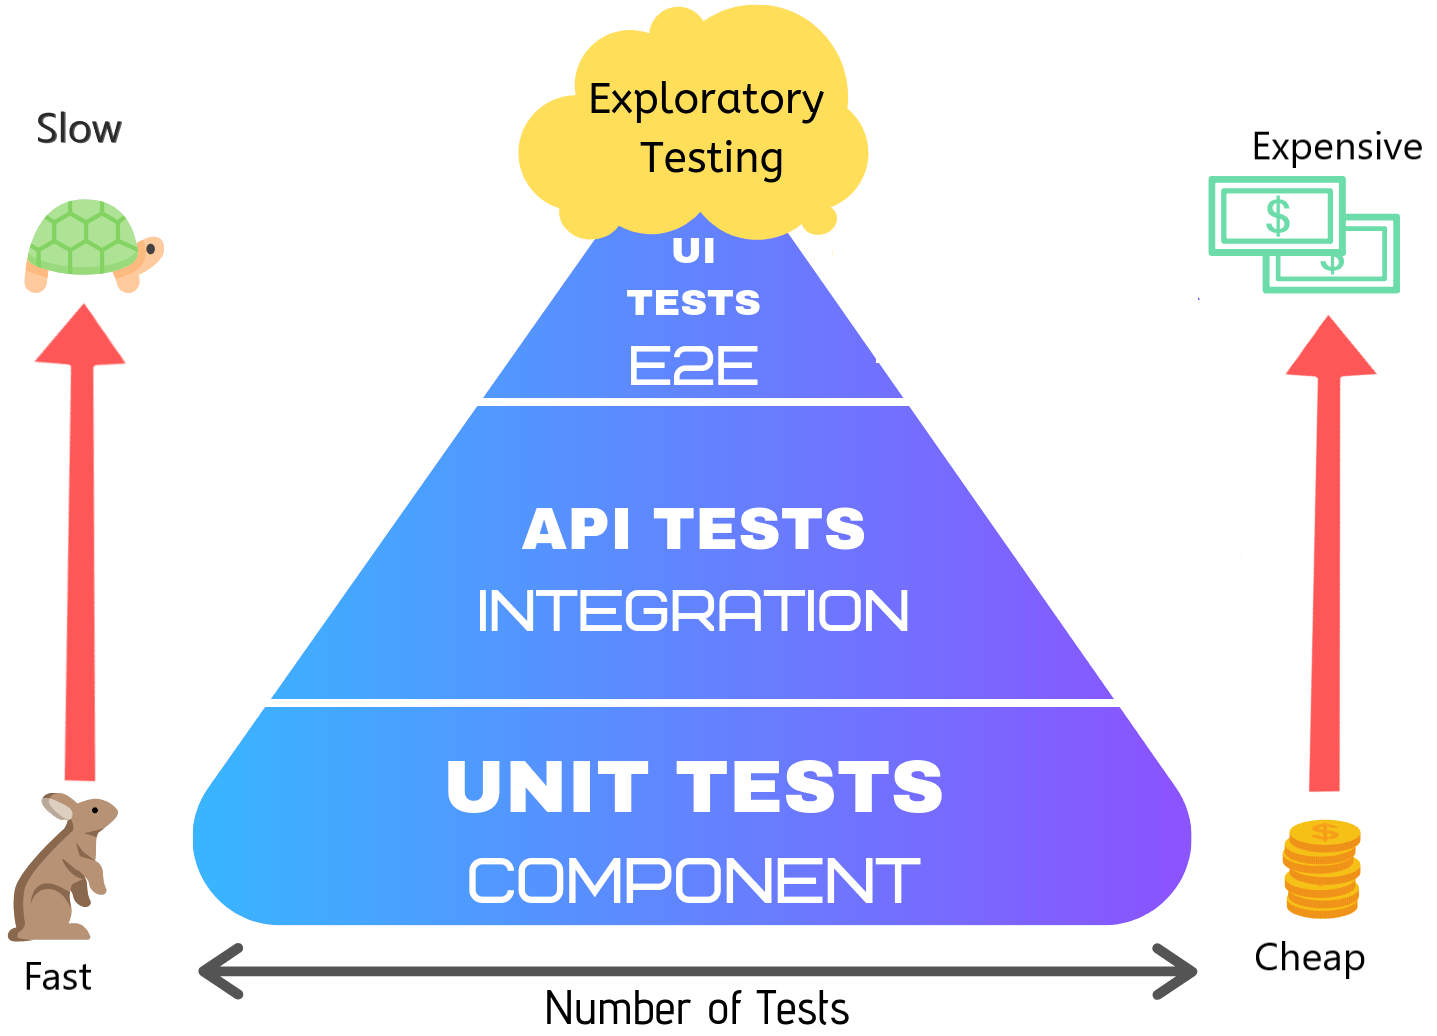
\includegraphics[scale=0.3]{piramideTest.png}
		\caption{Piramide dei test}\label{fig:test}
	\end{center}
\end{figure}

Come mostra la Figura~\ref{fig:test}, la piramide dei \emph{test} illustra il numero proporzionale di \emph{test} per ogni tipologia di \emph{test} in relazione alla loro velocità d'esecuzione e costi per implementarli. Sebbene i \emph{test} \gls{test e2e} forniscano un grande supporto per testare la correttezza dell'applicazione, sono significativamente più lenti e più costosi rispetto ai test unitari, a causa della loro elevata complessità e onerosità computazionale. Perciò è fondamentale trovare il giusto equilibrio di \emph{test} \gls{test e2e} da implementare senza perderne i vantaggi e senza aumentare i costi per l'implementazione. Una buona applicazione di \emph{test} \gls{test e2e} può essere ad esempio il \emph{testing} di azioni ripetitive che grazie alla fatto che sono \emph{test} automatizzati, risultano essere meno costosi è più efficaci rispetto ai \emph{test} manuali.

\section{Ambiente di Testing}

\section{Test eseguiti}
